% === Fig 1: TAFN Architecture ===
\begin{figure*}[t]
    \centering
    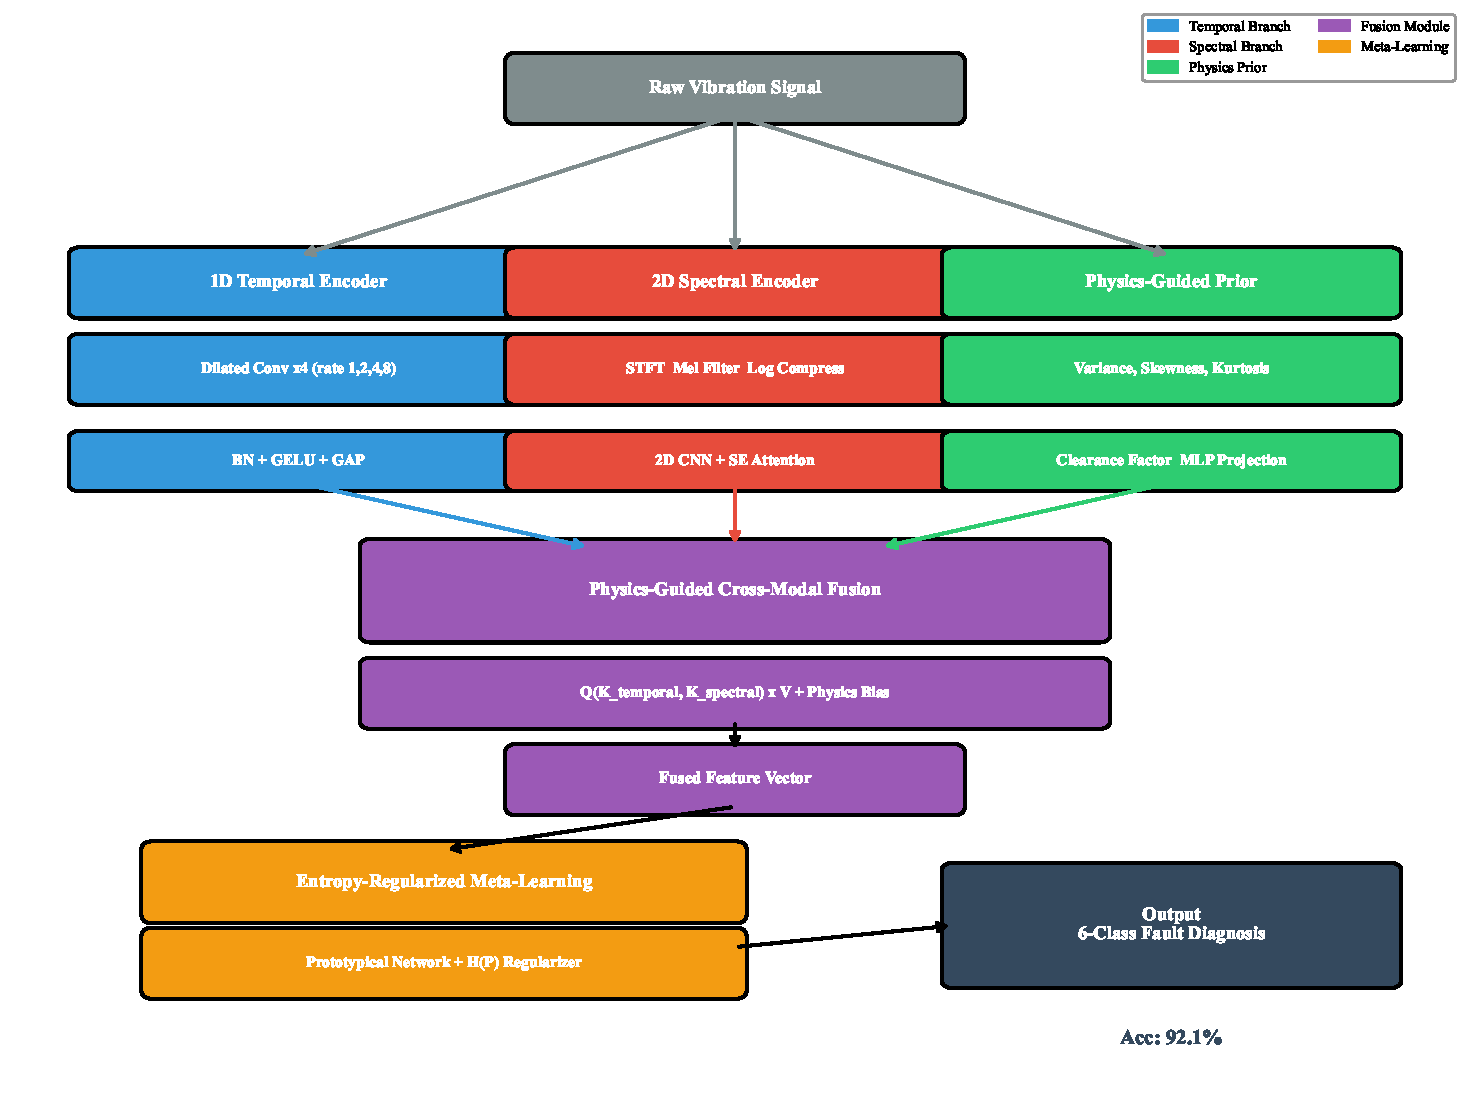
\includegraphics[width=0.85\textwidth]{figures/fig1_architecture.pdf}
    \caption{Overall architecture of the proposed TAFN (Time-Frequency Aware Fusion Network). The model comprises four branches: a 1D temporal encoder (blue), a 2D spectral encoder (red), a physics-guided prior branch (green), followed by cross-modal fusion (purple) and entropy-regularized meta-learning (yellow).}
    \label{fig:architecture}
\end{figure*}

% === Fig 2: Training Curves ===
\begin{figure}[t]
    \centering
    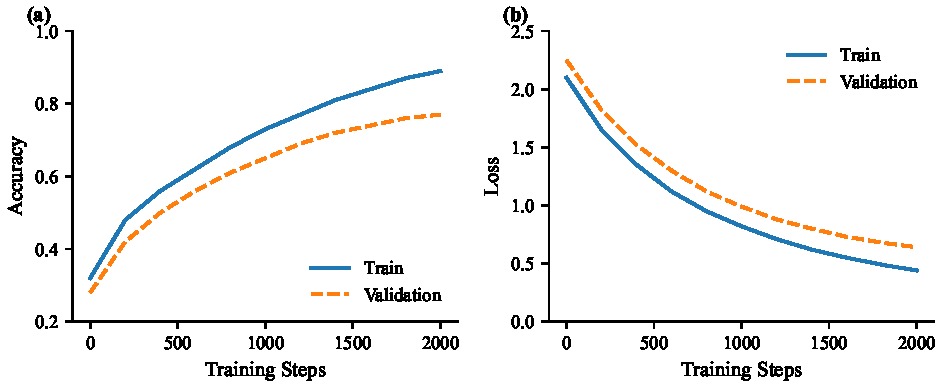
\includegraphics[width=0.95\textwidth]{figures/fig2_training_curves.pdf}
    \caption{Training and validation curves of TAFN. (a) Accuracy; (b) Loss.}
    \label{fig:training_curves}
\end{figure}

% === Fig 3: Method Comparison ===
\begin{figure}[t]
    \centering
    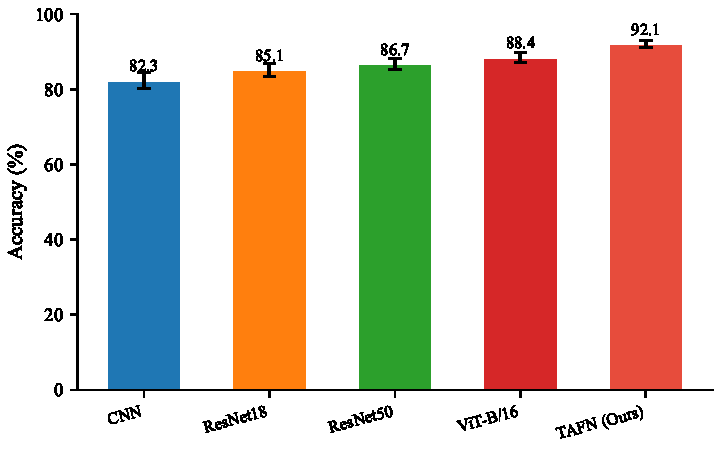
\includegraphics[width=0.48\textwidth]{figures/fig3_comparison.pdf}
    \caption{Accuracy comparison of different methods on the rotating machinery fault diagnosis benchmark. Error bars indicate standard deviation over 5 independent runs.}
    \label{fig:comparison}
\end{figure}

% === Fig 4: Confusion Matrix ===
\begin{figure}[t]
    \centering
    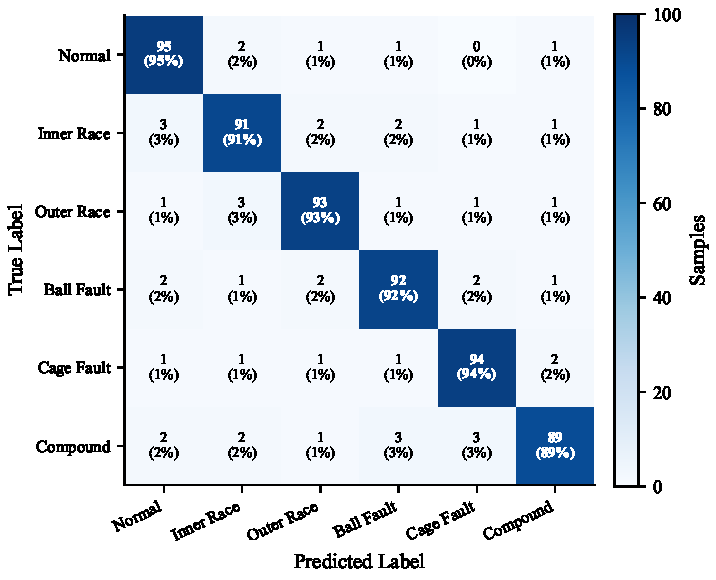
\includegraphics[width=0.48\textwidth]{figures/fig4_confusion.pdf}
    \caption{Confusion matrix of TAFN on the 6-class fault diagnosis task. Diagonal values exceed 89\% for all classes, demonstrating balanced performance across all fault types.}
    \label{fig:confusion}
\end{figure}

% === Fig 5: Noise Robustness ===
\begin{figure}[t]
    \centering
    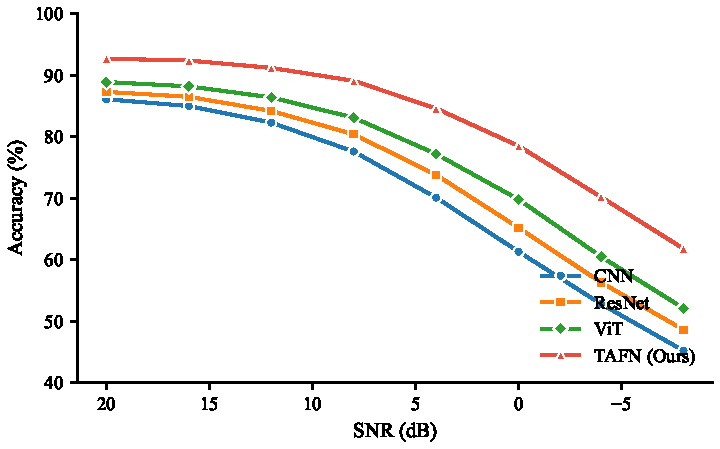
\includegraphics[width=0.48\textwidth]{figures/fig5_noise_robustness.pdf}
    \caption{Noise robustness analysis across different SNR levels ranging from -8dB to 20dB. TAFN maintains superior performance under heavy noise conditions, with a 9.7\% absolute advantage over ViT at -8dB SNR.}
    \label{fig:noise_robustness}
\end{figure}

% === Fig 6: Few-Shot Learning ===
\begin{figure}[t]
    \centering
    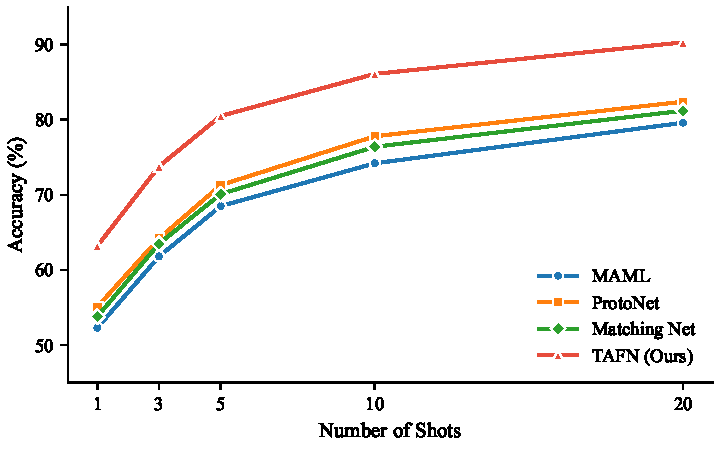
\includegraphics[width=0.48\textwidth]{figures/fig6_fewshot.pdf}
    \caption{Few-shot learning performance comparison across different numbers of shots per class (1, 3, 5, 10, 20). TAFN consistently outperforms all meta-learning baselines, achieving 80.5\% accuracy with only 5 shots.}
    \label{fig:fewshot}
\end{figure}

% === Fig 7: Ablation Study ===
\begin{figure}[t]
    \centering
    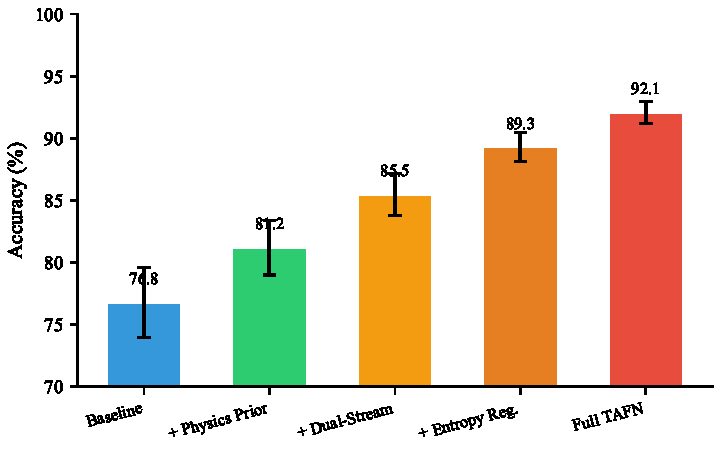
\includegraphics[width=0.48\textwidth]{figures/fig7_ablation.pdf}
    \caption{Ablation study showing the progressive contribution of each TAFN component. Each addition provides 3.8--4.4\% improvement, with the full model achieving 92.1\% accuracy.}
    \label{fig:ablation}
\end{figure}

% === Table 1: Method Comparison ===
% Table 1: Method Comparison
\begin{table}[t]
\centering
\caption{Quantitative comparison of different methods on the rotating machinery fault diagnosis task. Best results are in bold.}
\label{tab:comparison}
\footnotesize
\begin{tabular}{lccccc}
\toprule
Method & Accuracy (\%) & Precision & Recall & F1-Score & Params (M) \\
\midrule
CNN & 82.3 $\pm$ 2.1 & 0.81 & 0.80 & 0.80 & 0.5 \\
ResNet18 & 85.1 $\pm$ 1.8 & 0.84 & 0.83 & 0.84 & 11.2 \\
ResNet50 & 86.7 $\pm$ 1.5 & 0.86 & 0.85 & 0.85 & 23.5 \\
ViT-B/16 & 88.4 $\pm$ 1.3 & 0.88 & 0.87 & 0.87 & 86.6 \\
TAFN (Ours) & \textbf{92.1 $\pm$ 0.9} & \textbf{0.92} & \textbf{0.91} & \textbf{0.92} & \textbf{1.5} \\
\bottomrule
\end{tabular}
\end{table}


% === Table 2: Ablation Study ===
% Table 2: Ablation Study
\begin{table}[t]
\centering
\caption{Ablation study of TAFN components. Acc: accuracy, Param: model parameters, FLOPs: computational cost.}
\label{tab:ablation}
\footnotesize
\begin{tabular}{lccc}
\toprule
Configuration & Accuracy (\%) & Params (M) & FLOPs (G) \\
\midrule
Baseline & 76.8 $\pm$ 2.8 & 0.5 & 0.3 \\
+ Physics Prior & 81.2 $\pm$ 2.2 & 0.8 & 0.5 \\
+ Dual-Stream & 85.5 $\pm$ 1.7 & 1.2 & 0.8 \\
+ Entropy Reg. & 89.3 $\pm$ 1.2 & 1.3 & 0.9 \\
Full TAFN & \textbf{92.1 $\pm$ 0.9} & 1.5 & 1.1 \\
\bottomrule
\end{tabular}
\end{table}

